\chapter{Конструкторская часть}

\section{Разработка алгоритмов сортировки}

На рисунках \ref{pss1} -- \ref{sss} представлены схемы исследуемых алгоритмов сортировки.

\begin{figure}[h]
	\centering
	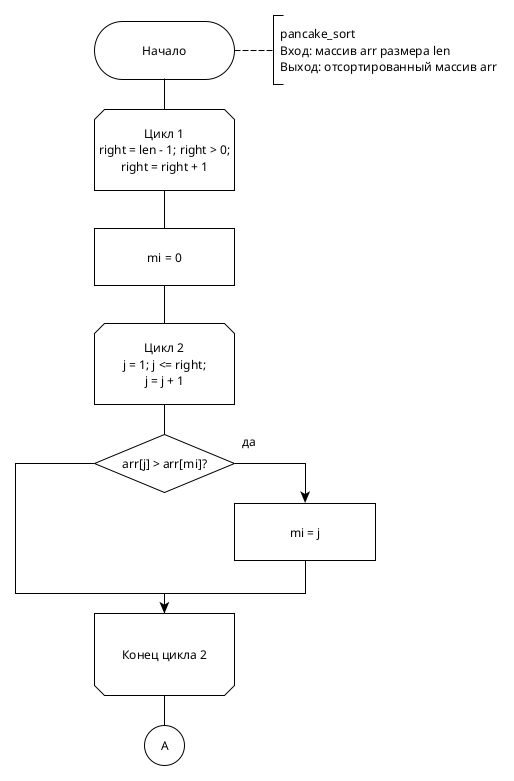
\includegraphics[width=0.9\linewidth]{pancakesort1}
	\caption{Cхема алгоритма блинной сортировки}
	\label{pss1}
\end{figure}

\begin{figure}[h]
	\centering
	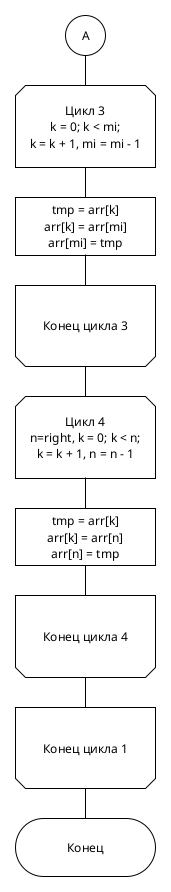
\includegraphics[width=0.25\linewidth]{pancakesort2}
	\caption{Cхема алгоритма блинной сортировки}
	\label{pss2}
\end{figure}

\begin{figure}[h]
	\centering
	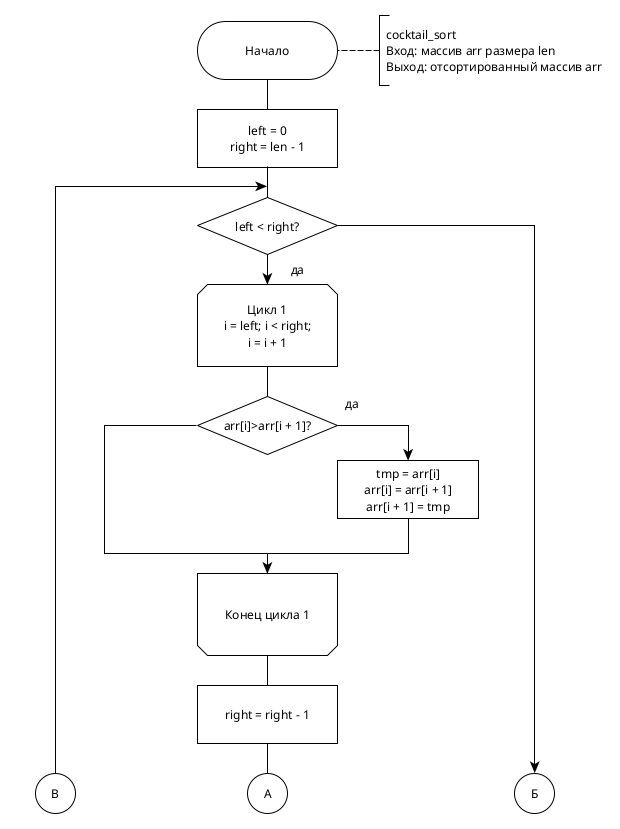
\includegraphics[width=0.9\linewidth]{cocktailsort1}
	\caption{Cхема алгоритма сортировки перемешиванием}
	\label{css1}
\end{figure}

\begin{figure}[h]
	\centering
	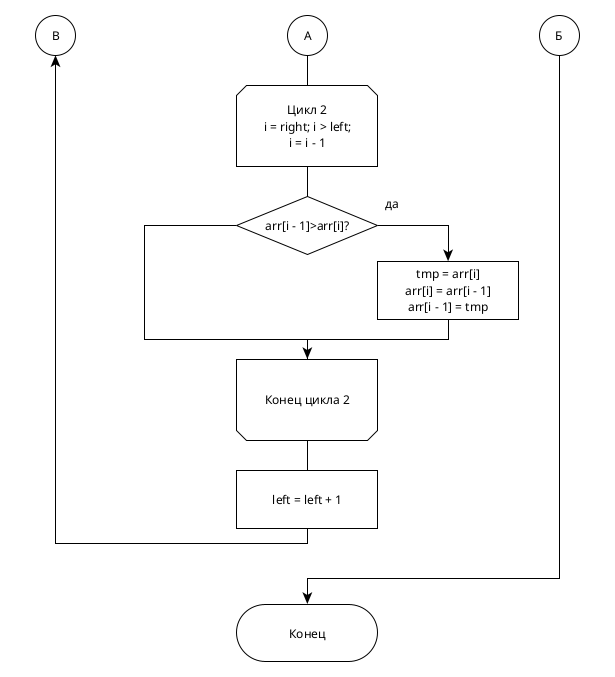
\includegraphics[width=0.9\linewidth]{cocktailsort2}
	\caption{Cхема алгоритма сортировки перемешиванием}
	\label{css2}
\end{figure}

\begin{figure}[h]
	\centering
	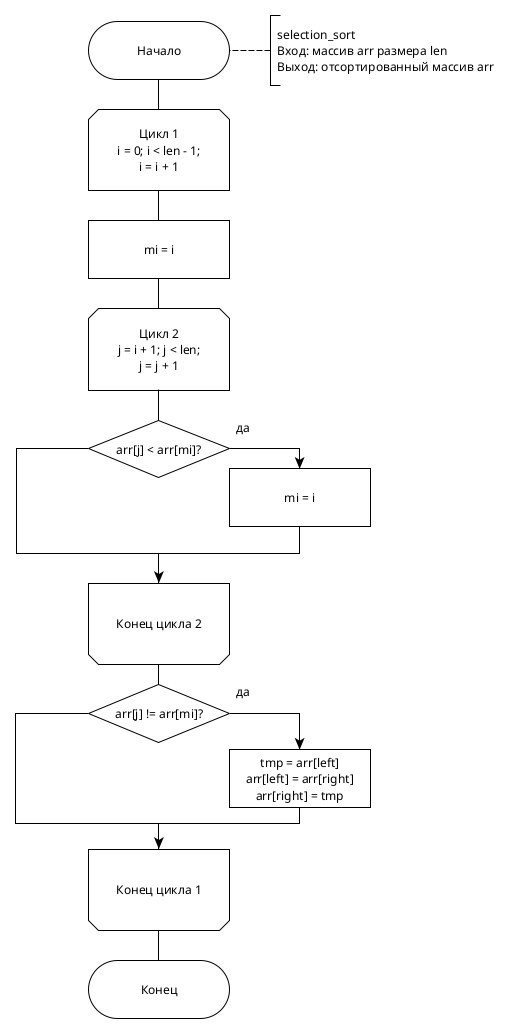
\includegraphics[width=0.65\linewidth]{selectionsort}
	\caption{Cхема алгоритма сортировки выбором}
	\label{sss}
\end{figure}

\section{Оценка трудоемкости алгоритмов сортировки}

Для оценки трудоемкости алгоритмов сортировки используется следующая модель:

\begin{itemize}
	\item Трудоемкость операций
	\begin{equation}\label{o1}
	>>, <<, [], +, -, =, +=, -=, ==, <, >, <=, >=, !=, ++, --
	\end{equation}
	единична;
	\item Трудоемкость операций
	\begin{equation}\label{o2}
		*, \%, /
	\end{equation}
	равна 2;
	\item Трудоемкость условного оператора вычисляется по формуле:
	\begin{equation}\label{oif}
		f_{if} = f_{cond} + 
		\begin{cases}
			min(f_1, f_2), & \text{лучший случай}, \\
			max(f_1, f_2), & \text{худший случай},
		\end{cases}
	\end{equation}
	где $f_{cond}$ - трудоемкость проверки условия,\\\text{~~~~~}$f_1$ - трудоемкость тела условного оператора, если выполняется условие;\\\text{~~~~~}$f_2$ - трудоемкость тела условного оператора, если условие не выполняется.
	\item Трудоемкость цикла вычисляется по формуле:
	\begin{equation}\label{oc}
	f_c = f_{init} + f_{comp} + N(f_{body} + f_{inc} + f_{comp}),
	\end{equation}
	где $f_{init}$ - трудоемкость инициализации счетчика цикла,\\\text{~~~~~}$f_{comp}$ - трудоемкость проверки условия цикла,\\\text{~~~~~}$f_{body}$ - трудоемкость тела цикла,\\\text{~~~~~}$f_{inc}$ - трудоемкость инкремента счетчика цикла,\\\text{~~~~~}$N$ - количество итераций.
\end{itemize}

\subsection{Алгоритм блинной сортировки}

Оценим трудоемкость алгоритма блинной сортировки.

Трудоемкость условного оператора внутри цикла 2 определяется следующим образом:
\begin{equation}\label{psif1}
	f_{if1} =
	\begin{cases}
		3, & \text{лучший случай}, \\
		4, & \text{худший случай}.
	\end{cases}.
\end{equation}

Используя формулы\text{~}\eqref{oc}\text{~}и\text{~}\eqref{psif1}, определим суммарную трудоемкость цикла 2 для лучшего и худшего случаев:
\begin{equation}\label{psc2b}
	f_{c2_{best}} = (N - 1)(1 + 1) + \frac{N(N - 1)}{2}(f_{if1} + 2 + 1) = 3N^2 - N - 2,
\end{equation}
\begin{equation}\label{psc2w}
	f_{c2_{worst}} = (N - 1)(1 + 1) + \frac{N(N - 1)}{2}(f_{if1} + 2 + 1) = \frac{7}{2}N^2 - \frac{1}{2}N - 2.
\end{equation}

Трудоемкость цикла 4 вычисляется по формуле\text{~}\eqref{oc}:
\begin{equation}\label{psc4}
	f_{c4} = 1 + 1 + 1 + \floor{\frac{N}{2}}(7 + 1 + 2 + 2) = 6N + 3.
\end{equation}

Вычислим суммарную трудоемкость цикла 3 для лучшего случая. Для него характерна ситуация, при которой значение переменной $mi = 0$. Очевидно, что в лучшем случае суммарная трудоемкость цикла 3 будет равна:
\begin{equation}\label{psc3b}
	f_{c3_{best}} = (1 + 1)(N - 1) = 2N - 2.
\end{equation}

Определим суммарную трудоемкость цикла 3 для худшего случая. Для него характерна ситуация, при которой переменная $mi$ равна $right$ после работы цикла 2. Тогда суммарное количество итераций цикла 3 равно:
\begin{equation}\label{psc3wi}
	k_{c4_{worst}} = \floor{\frac{N}{2}}, \floor{\frac{N - 1}{2}}, ... 2, 1.
\end{equation}

Если значение N нечетно, то формула\text{~}\eqref{psc3wi} примет вид:
\begin{equation}\label{psc3wio}
	k_{c4_{worst}} = \frac{N - 1}{2} + \frac{N - 1}{2} + \frac{N - 3}{2} + \frac{N - 1}{2} + ... + 2 + 2 + 1 + 1 = \frac{N^2 - 1}{4}.
\end{equation}

Если же значение N четно, то формула\text{~}\eqref{psc3wi} примет вид:
\begin{equation}\label{psc3wie}
	k_{c4_{worst}} = \frac{(N - 1)^2 - 1}{4} + \frac{N}{2} = \frac{N^2}{4}.
\end{equation}

Очевидно, что при нечетном значении N формула\text{~}\eqref{psc3wie} описывает наиболее трудоемкую ситуацию. Поэтому, используя формулы\text{~}\eqref{oc}\text{~}и\text{~}\eqref{psc3wie}, расcчитаем суммарную трудоемкость цикла 3 для худшего случая:
\begin{equation}\label{psc3w}
	f_{c3_{worst}} = (N - 1)(1 + 1) + k_{c4_{worst}}(2 + 3 + 2 + 2 + 2 + 1) = 3N^2 + 2N - 2.
\end{equation}

В итоге, используя формулы\text{~}\eqref{oc},\text{~}\eqref{psc2b},\text{~}\eqref{psc2w}\text{~}и\text{~}\eqref{psc4}, мы можем получить трудоемкость алгоритма блинной сортировки для лучшего и худшего случаев:
\begin{equation}\label{psb}
	f_{best} = f_{c1_{best}} = 2 + 1 + (N - 1)(1 + f_{c4} + 2) + f_{c2_{best}} + f_{c3_{best}} = 9N^2 + N - 7 = O(N^2),
\end{equation}
\begin{equation}\label{psw}
	f_{worst} = f_{c1_{worst}} = 2 + 1 + (N - 1)(1 + f_{c4} + 2) + f_{c2_{worst}} + f_{c3_{worst}} = \frac{25}{2}N^2 + \frac{3}{2}N - 7 = O(N^2).
\end{equation}

\subsection{Алгоритм сортировки перемешиванием}

Оценим трудоемкость алгоритма сортировки перемешиванием.

Трудоемкости условных операторов во внутренних циклах for определяются формулой\text{~}\eqref{oif}:
\begin{equation}\label{csif}
	f_{if1} = f_{if2} = f_{if} =
	\begin{cases}
		4, &\text{лучший случай}, \\
		13, &\text{худший случай}.
	\end{cases}.
\end{equation}

Используя формулы\text{~}\eqref{oc}\text{~}и\text{~}\eqref{csif}, определим суммарную трудоемкость внутренних циклов for для лучшего и худшего случаев:
\begin{equation}\label{csc2b}
	f_{c2_{best}} = (1 + 1 + 1 + 1)(N - 1) + \frac{N(N - 1)}{2}(2 + 1 + f_{if}) = \frac{7}{2}N^2 + \frac{1}{2}N - 4,
\end{equation}
\begin{equation}\label{csc2w}
	f_{c2_{worst}} = (1 + 1 + 1 + 1)(N - 1) + \frac{N(N - 1)}{2}(2 + 1 + f_{if}) = 8N^2 - 4N - 4.
\end{equation}

Используя формулы\text{~}\eqref{oc},\text{~}\eqref{csc2b}\text{~}и\text{~}\eqref{csc2w}, определим трудоемкость цикла while для лучшего и худшего случаев:
\begin{equation}\label{csc1b}
	f_{c1_{best}} = 1 + (N - 1)(2 + 2) + f_{c2_{best}} = \frac{7}{2}N^2 + \frac{9}{2}N - 7,
\end{equation}
\begin{equation}\label{csc1w}
	f_{c1_{worst}} = 1 + (N - 1)(2 + 2) + f_{c2_{worst}} = 8N^2 - 7.
\end{equation}

В итоге, применяя формулы text{~}\eqref{csc1b}\text{~}и\text{~}\eqref{csc1w}, мы можем вычислить трудоемкость алгоритма перемешиванием для лучшего и худшего случаев:
\begin{equation}\label{csb}
	f_{best} = 1 + 2 + f_{c1_{best}} = \frac{7}{2}N^2 + \frac{9}{2}N - 4 = O(N^2),
\end{equation}
\begin{equation}\label{csw}
	f_{worst} = 1 + 2 + f_{c1_{worst}} = 8N^2 - 4 = O(N^2).
\end{equation}

\subsection{Алгоритм сортировки выбором}

Оценим трудоемкость алгоритма сортировки выбором.

Трудоемкость условного оператора во внешнем цикле определяем по формуле\text{~}\eqref{oc}:
\begin{equation}\label{ssif1}
	f_{if1} = 
	\begin{cases}
		3, & \text{лучший случай}, \\
		10, & \text{худший случай}.
	\end{cases}
\end{equation}

По формуле\text{~}\eqref{oif} получаем трудоемкость условного оператора во внутреннем цикле:
\begin{equation}\label{ssif2}
	f_{if2} = 
	\begin{cases}
		3, & \text{лучший случай}, \\
		4, & \text{худший случай}.
	\end{cases}
\end{equation}

Используя формулы\text{~}\eqref{oc}\text{~}и\text{~}\eqref{ssif2}, определяем суммарную трудоемкость внутренних циклов для лучшего и худшего случаев:
\begin{equation}\label{ssc2b}
	f_{c2_{best}} = (2 + 1)(N - 1) + \frac{N(N - 1)}{2}(f_{if2} + 2 + 1) = 3N^2 - 3,
\end{equation}
\begin{equation}\label{ssc2w}
	f_{c2_{worst}} = (2 + 1)(N - 1) + \frac{N(N - 1)}{2}(f_{if2} + 2 + 1) = \frac{7}{2}N^2 - \frac{1}{2}N - 3.
\end{equation}

По формулам\text{~}\eqref{oc},\text{~}\eqref{ssif1},\text{~}\eqref{ssc2b}\text{~}и\text{~}\eqref{ssc2w} определяем трудоемкость внешнего цикла для лучшего и худшего случаев:
\begin{equation}\label{ssc1b}
	f_{c1_{best}} = 3 + (N - 1)(2 + 2 + 1 + f_{if1}) + f_{c2_{best}} = 3N^2 + 8N - 8,
\end{equation}
\begin{equation}\label{ssc1w}
	f_{c1_{worst}} = 3 + (N - 1)(2 + 2 + 1 + f_{if1}) + f_{c2_{worst}} = \frac{7}{2}N^2 + \frac{29}{2}N - 15.
\end{equation}

В итоге, по формулам\text{~}\eqref{ssc1b}\text{~}и\text{~}\eqref{ssc1w} получаем трудоемкость алгоритма сортировки выбором. Для лучшего случая:
\begin{equation}\label{ssb}
	f_{best} = 3N^2 + 8N - 8 = O(N^2).
\end{equation}
Для худшего случая:
\begin{equation}\label{ssw}
	f_{worst} = \frac{7}{2}N^2 + \frac{29}{2}N - 15 = O(N^2).
\end{equation}

\section*{Вывод}

В данном разделе были разработаны и оцененены трудоемкости следующих алгоритмов сортировки: блинной, перемешиванием и выбором.

Результаты оценки:
\begin{itemize}
	\item блинная сортировка: $f_{best} = O(N^2)$, $f_{worst} = O(N^2)$;
	\item сортировка перемешиванием: $f_{best} = O(N^2)$, $f_{worst} = O(N^2)$;
	\item сортировка выбором: $f_{best} = O(N^2)$, $f_{worst} = O(N^2)$.
\end{itemize}

\clearpage
